%!TEX root = main.tex
\documentclass[letterpaper, 12pt]{extarticle}
% \usepackage{fontspec}
% ==================================================

% document parameters
% \usepackage[spanish, mexico, es-lcroman]{babel}
\usepackage[spanish]{babel}
\decimalpoint
\usepackage[margin = 0.7in]{geometry}

% ==================================================

% Packages for math
\usepackage{cancel} % Agregar en el preámbulo
\usepackage{mathrsfs}
\usepackage{amsfonts}
\usepackage{amsmath}
\usepackage{amsthm}
\usepackage{amssymb}
\usepackage{physics}
\usepackage{dsfont}
\usepackage{esint}
% ==================================================

% Packages for writing
\usepackage{enumerate}
\usepackage[shortlabels]{enumitem}
\usepackage{framed}
\usepackage{csquotes}

% ==================================================

% Miscellaneous packages
\usepackage{float}
\usepackage{tabularx}
\usepackage{listings}
\usepackage{xcolor}
\usepackage{multicol}
\usepackage{subcaption}
\usepackage{caption}
\captionsetup{format = hang, margin = 10pt, font = small, labelfont = bf}

\lstset{
	language=Matlab,
	basicstyle=\ttfamily\footnotesize,
	keywordstyle=\color{blue},
	commentstyle=\color{gray},
	stringstyle=\color{red},
	numbers=left,
	numberstyle=\tiny,
	stepnumber=1,
	numbersep=5pt,
	frame=single,
	rulecolor=\color{black}
}

% Citation
\usepackage[round, authoryear]{natbib}

% Hyperlinks setup
\usepackage{hyperref}
\definecolor{links}{rgb}{0.36,0.54,0.66}
\hypersetup{
	colorlinks = true,
	linkcolor = black,
	urlcolor = blue,
	citecolor = blue,
	filecolor = blue,
	pdfauthor = {Author},
	pdftitle = {Title},
	pdfsubject = {subject},
	pdfkeywords = {one, two},
	pdfproducer = {LaTeX},
	pdfcreator = {pdfLaTeX},
} 
\usepackage{titlesec}
\usepackage[many]{tcolorbox}

% Adjust spacing after the chapter title
\titlespacing*{\chapter}{0cm}{-2.0cm}{0.50cm}
\titlespacing*{\section}{0cm}{0.50cm}{0.25cm}

% Indent 
\setlength{\parindent}{0pt}
\setlength{\parskip}{1ex}

% --- Theorems, lemma, corollary, postulate, definition ---
% \numberwithin{equation}{section}

\newtcbtheorem[]{problem}{Problem}%
    {enhanced,
    colback = black!5, %white,
    colbacktitle = black!5,
    coltitle = black,
    boxrule = 0pt,
    frame hidden,
    borderline west = {0.5mm}{0.0mm}{black},
    fonttitle = \bfseries,
    breakable,
    before skip = 3ex,
    after skip = 3ex
}{problem}

\newtcbtheorem[no counter]{solution}{Solution}%
    {enhanced,
    colback = white,
    colbacktitle = white,
    coltitle = black,
    boxrule = 0pt,
    frame hidden,
    borderline west = {0.5mm}{0.0mm}{blue},
    fonttitle = \bfseries,
    breakable,
    before skip = 3ex,
    after skip = 3ex
}{solution}

\tcbuselibrary{skins, breakable}

% --- You can define your own color box. Just copy the previous \newtcbtheorm definition and use the colors of yout liking and the title you want to use.
% --- Basic commands ---
%   Euler's constant
\newcommand{\eu}{\mathrm{e}}

%   Imaginary unit
\newcommand{\im}{\mathrm{i}}

%   Sexagesimal degree symbol
\newcommand{\grado}{\,^{\circ}}

% --- Comandos para álgebra lineal ---
% Matrix transpose
\newcommand{\transpose}[1]{{#1}^{\mathsf{T}}}

%%% Comandos para cálculo
%   Definite integral from -\infty to +\infty
\newcommand{\Int}{\int\limits_{-\infty}^{\infty}}

%   Indefinite integral
\newcommand{\rint}[2]{\int{#1}\dd{#2}}

%  Definite integral
\newcommand{\Rint}[4]{\int\limits_{#1}^{#2}{#3}\dd{#4}}

%   Dot product symbol (use the command \bigcdot)
\makeatletter
\newcommand*\bigcdot{\mathpalette\bigcdot@{.5}}
\newcommand*\bigcdot@[2]{\mathbin{\vcenter{\hbox{\scalebox{#2}{$\m@th#1\bullet$}}}}}
\makeatother

%   Hamiltonian
\newcommand{\Ham}{\hat{\mathcal{H}}}

%   Trace
\renewcommand{\Tr}{\mathrm{Tr}}

% Christoffel symbol of the second kind
\newcommand{\christoffelsecond}[4]{\dfrac{1}{2}g^{#3 #4}(\partial_{#1} g_{#2 #4} + \partial_{#2} g_{#1 #4} - \partial_{#4} g_{#1 #2})}

% Riemann curvature tensor
\newcommand{\riemanncurvature}[5]{\partial_{#3} \Gamma_{#4 #2}^{#1} - \partial_{#4} \Gamma_{#3 #2}^{#1} + \Gamma_{#3 #5}^{#1} \Gamma_{#4 #2}^{#5} - \Gamma_{#4 #5}^{#1} \Gamma_{#3 #2}^{#5}}

% Covariant Riemann curvature tensor
\newcommand{\covariantriemanncurvature}[5]{g_{#1 #5} R^{#5}{}_{#2 #3 #4}}

% Ricci tensor
\newcommand{\riccitensor}[5]{g_{#1 #5} R^{#5}{}_{#2 #3 #4}}

\begin{document}

\begin{Large}
	\textbf{\textbf{Tarea 1}}

	Control por Modos Deslizantes
\end{Large}

\vspace{1ex}

\textbf{Student:} \text{Alejandro León}, \href{mailto:j.alejandro.ls00@gmail.com}{\texttt{j.alejandro.ls00@gmail.com}}\\
\textbf{Profesor:} \text{Dr. Leonid Fridman} \\
\textbf{Due Date:} Apr 24, 2025 \\

\vspace{2ex}

\textbf{Solve exercises 1.2, 1.7, 2.1, 2.2, 2.3, 2.5}

\begin{problem}{1.1}{problem1_1}

A simplified $m$ longitudinal motion of an underwater vehicle can be described by
\begin{equation}
	m \ddot{x} + k \dot{x} |\dot{x}| = u
\end{equation}
where $x$ is the position of the vehicle, $u$ is the control input (a force that is provided by a propeller), $m$ is the mass of the vehicle, and $k > 0$ is the drag coefficient. Assuming the value of $m$ is known exactly, the drag coefficient is bounded $k_1 \leq k \leq k_2$, and the position and its derivative (velocity) $x, \dot{x}$ are measured:

\begin{enumerate}[label=\textbf{\alph*)}]
	\item Obtain a state system model of the vehicle using $x_1 = x, \, x_2 = \dot{x}$ as the state variables.
	\item Design a conventional sliding mode control law $u$ that drives $x_1, x_2 \rightarrow 0$ as time increases.
	\item Simulate the control system for $x_1(0) = 2\,\text{m}$, $x_2(0) = 0.5\,\text{m/s}$, $m = 4\,\text{kg}$, and $k = 1.5 + 0.4 \sin(2t)\,[\text{kg/ms}]$. Plot the time histories of the sliding variable, the control function $u$, the position $x_1$, and the velocity $x_2$.
	\item Identify the quantities that reach zero in finite time and the ones that approach zero asymptotically.
\end{enumerate}

\textbf{Hint:} The function $k\dot{x}|\dot{x}|$ can be bounded as
\[
	|k\dot{x}|\dot{x}|| \leq k_2 \dot{x}^2 = 1.9 \dot{x}^2.
\]

\end{problem}

\begin{solution}{}{solution1_1}
	\begin{enumerate}[label=\textbf{\alph*)}]
		\item Using the state variables \( x_1 = x \) and \( x_2 = \dot{x} \), the dynamic model of the vehicle can be expressed as:

		      \begin{equation*}
			      \begin{aligned}
				      \dot{x}_1 & = x_2,                                         \\
				      \dot{x}_2 & = \frac{1}{m} \left( -k x_2 |x_2| + u \right).
			      \end{aligned}
		      \end{equation*}

		\item Define the sliding surface as:
		      \[
			      \sigma = x_2 + c x_1, \quad c > 0,
		      \]
		      with its time derivative given by:
		      \[
			      \dot{\sigma} = c \dot{x}_1 + \dot{x}_2 = c x_2 + \frac{1}{m} \left( -k x_2 |x_2| + u \right).
		      \]

		      Consider the following Lyapunov candidate function:
		      \[
			      V = \frac{1}{2} \sigma^2,
		      \]
		      which has the time derivative:
		      \[
			      \dot{V} = \sigma \dot{\sigma} = \sigma \left( c x_2 + \frac{1}{m} \left( -k x_2 |x_2| + u \right) \right).
		      \]

		      Choose the control input as:
		      \[
			      u = m(-c x_2 + v),
		      \]
		      so that:
		      \[
			      \dot{V} = \sigma \left( -\frac{k}{m} x_2 |x_2| + v \right).
		      \]

		      Using the provided bound on the nonlinear term from the hint:
		      \[
			      |k x_2 |x_2|| \leq k_2 x_2^2 = 1.9 x_2^2,
		      \]
		      we can bound the derivative of \( V \) as:
		      \[
			      \dot{V} \leq |\sigma| \frac{1.9}{m} x_2^2 + \sigma v.
		      \]

		      To dominate the first term and ensure convergence, choose:
		      \[
			      v = -\left( \rho + \frac{1.9}{m} x_2^2 \right) \text{sign}(\sigma),
		      \]
		      where \( \rho > 0 \) is a design parameter.

		\item The simulation of the control system using $c=2$ and $\rho =2$ yields the following results:
		      \begin{figure}[H]
			      \centering
			      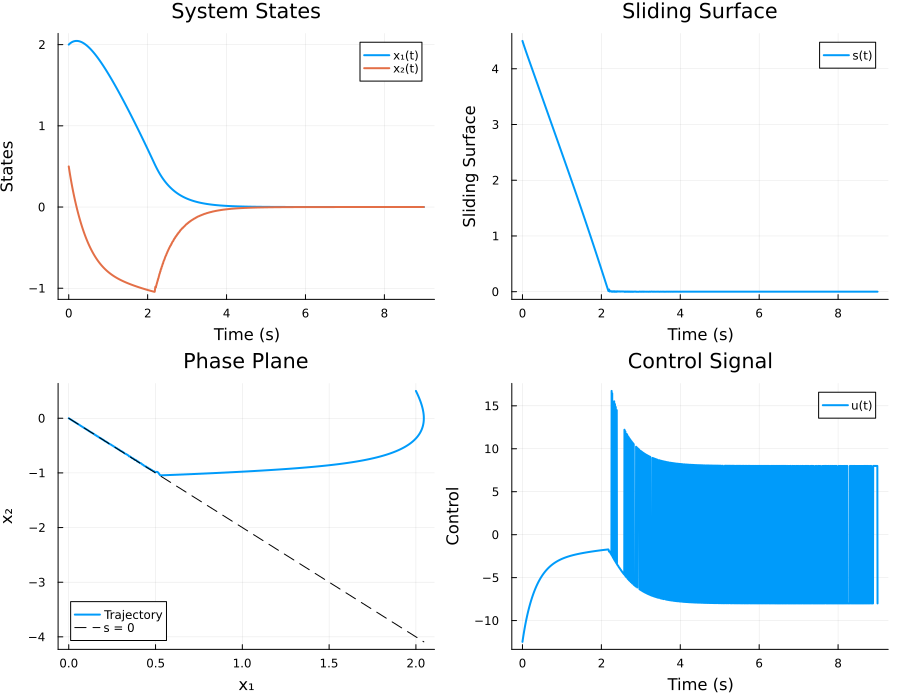
\includegraphics[width=1\textwidth]{img/problem1_1.png}
			      \caption{Simulation results for the sliding mode control system.}
			      \label{fig:problem1_1}
		      \end{figure}
        \item We can observe that the sliding variable \( \sigma \) reaches zero in finite time, indicating that the system enters the sliding mode, while the states \( x_1 \) and \( x_2 \) approach zero asymptotically. 

	\end{enumerate}
	\qed
\end{solution}
\newpage
\begin{problem}{1.2}{problem1_2}

Repeat Exercise 1.1 approximating the \textit{sign} funcion in the control law by the sigmoid function $\text{sign}(\sigma) \approx \frac{\sigma}{|\sigma| + \varepsilon}$ and separately by the saturation function
\[
	\text{sign}(\sigma) \approx
	\begin{cases}
		1                          & \text{if } \quad \sigma > \varepsilon,       \\
		\frac{\sigma}{\varepsilon} & \text{if } \quad  |\sigma| \leq \varepsilon, \\
		-1                         & \text{if } \quad  \sigma < -\varepsilon.
	\end{cases}
\]

\end{problem}

\begin{solution}{}{solution1_2}
	As the analysis is practically the same as in Exercise 1.1, we will only show the results for the sigmoid and saturation approximations, and a discussion of the results.
	\begin{enumerate}[label=\textbf{\alph*)}, start=3]
		\item \begin{enumerate}[label=\textbf{\roman*)}]
			      \item Using the saturation approximation, we have:
			            \[
				            u = m(-c x_2 + v) = m \left( -c x_2 - \left( \rho + \frac{1.9}{m} x_2^2 \right) \text{sat}(\sigma) \right).
			            \]

			            \begin{figure}[H]
				            \centering
				            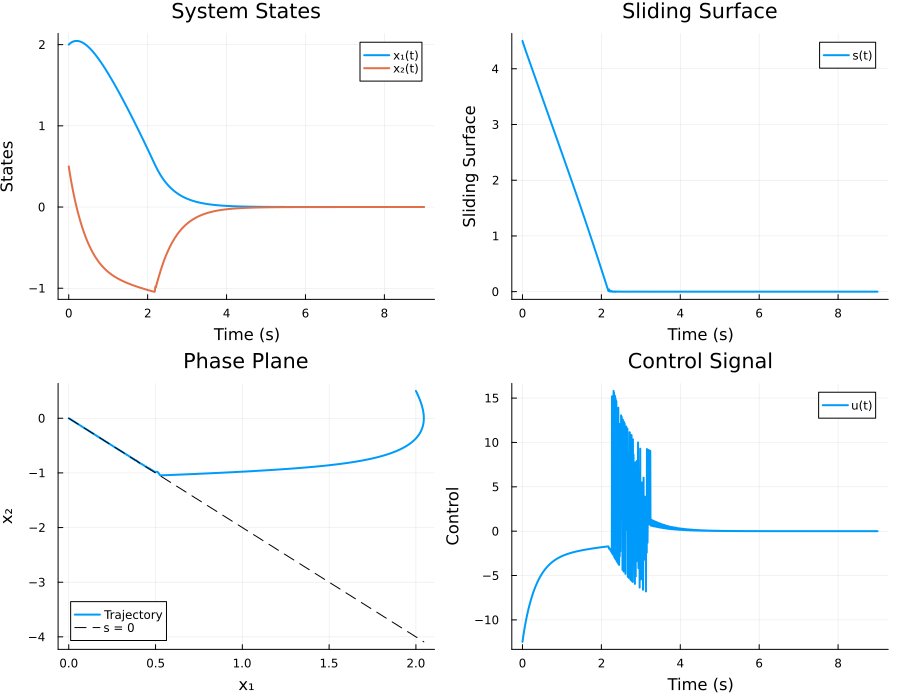
\includegraphics[width=1\textwidth]{img/problem1_2_sat.png}
				            \caption{Simulation results for the sliding mode control system using saturation approximation.}
				            \label{fig:problem1_2_sat}
			            \end{figure}

			      \item Using the sigmoid approximation, we have:
			            \[
				            u = m(-c x_2 + v) = m \left( -c x_2 - \left( \rho + \frac{1.9}{m} x_2^2 \right) \frac{\sigma}{|\sigma| + \varepsilon} \right).
			            \]

			            \begin{figure}[H]
				            \centering
				            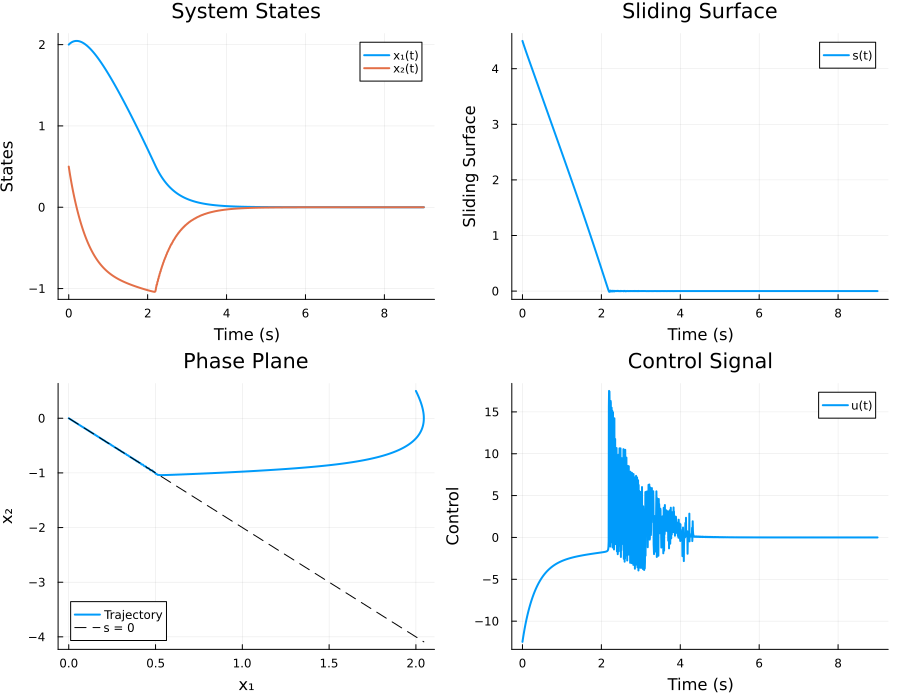
\includegraphics[width=1\textwidth]{img/problem1_2_sigmoid.png}
				            \caption{Simulation results for the sliding mode control system using sigmoid approximation.}
				            \label{fig:problem1_2_sig}
			            \end{figure}
		      \end{enumerate}
	\end{enumerate}
	In both cases, we can observe that the system seems to have finite time convergence in the sliding variable, and the chattering attenuation in the control input is evident. The saturation approximation leads to a more abrupt control action at the beginning, while the sigmoid approximation provides a smoother transition. Despite this, both approximations yield similar results in terms of system behavior and performance. It is clear that both approximations are effective in reducing chattering, but the theory suggests that both approximations only drive the sliding variable asymptotically to zero, so these are not ideal sliding modes, even though, in this case, and with that very small $\varepsilon$, the system behaves as if it were a sliding mode in both cases.
	\qed
\end{solution}
\newpage
\begin{problem}{1.6}{problem1_6}

For the DC motor modeled by
\begin{equation}
	\begin{aligned}
		J\frac{d\omega}{dt} & = k_m i - T_L,          \\
		L\frac{di}{dt}      & = -iR - k_b \omega + u,
	\end{aligned}
	\label{eq:dcmotor}
\end{equation}
where \( J \) is the moment of inertia, \( i \) is the armature current, \( L \) and \( R \) are the armature inductance and resistance respectively, \( \omega \) is the motor angular speed, \( k_b \) is a constant of back electromotive force, \( k_m \) is a motor torque constant, \( T_L \) is an unknown load torque which is bounded and has a bounded derivative, and \( u \) is a control function defined by the armature voltage.

Design a sliding mode control \( u \), steering the angular speed \( \omega \) to zero assuming both \( i \) and \( \omega \) are measurable and all parameters are known. Simulate the control system with the following parameters:
\[
	\begin{aligned}
		R         & = 1\,\Omega,                        \\
		L         & = 0.5\,\text{H},                    \\
		k_m       & = 5 \times 10^{-2}\,\text{Nm/A},    \\
		k_b       & = k_m,                              \\
		J         & = 10^{-3}\,\text{Nms}^2/\text{rad}, \\
		T_L       & = 0.1 \sin(t)\,\text{Nm},           \\
		\omega(0) & = 1\,\text{rad/s},                  \\
		i(0)      & = 0.
	\end{aligned}
\]

Plot the time histories of the sliding variable, the control function \( u \), the current \( i \), and the angular speed \( \omega \).

\end{problem}

\begin{solution}{}{solution1_6}
	The system \eqref{eq:dcmotor} can be represented in state-space form as:
	\[
		\begin{aligned}
			\dot{x}_1 & = \frac{k_m}{J} x_2 - \frac{T_L}{J}, \\
			\dot{x}_2 & = -\frac{k_b}{L} x_1 - \frac{R}{L} x_2 + \frac{1}{L} u,
		\end{aligned}
	\]
	where \( x_1 = \omega \) (angular speed) and \( x_2 = i \) (armature current).

	The control objective is to drive \( \omega = x_1 \to 0 \) as \( t \to \infty \). To this end, we define the sliding variable as
	\[
		\begin{aligned}
			s & = \dot{x}_1 + \lambda x_1 \\
			  & = \frac{k_m}{J} x_2 - \frac{T_L}{J} + \lambda x_1.
		\end{aligned}
	\]
	The term \( -\frac{T_L}{J} \) is considered as an unmatched disturbance, letś redefine the sliding variable as:
	\[
		s = \frac{k_m}{J} x_2 + \lambda x_1.
	\]

	On the sliding surface \( s = 0 \), the dynamics reduce to:
	\[
		x_2 = -\frac{\lambda J}{k_m} x_1.
	\]
	Substituting into the first state equation yields:
	\[
		\dot{x}_1 = -\lambda x_1 - \frac{T_L}{J}.
	\]
    Thus, the disturbance that enters in the first equation (where control is absent) will prevent the state variable from converging to zero in the sliding mode. Nevertheless, let's continue with the typical approach to see this fenomena.\\

	Consider the Lyapunov candidate:
	\[
		V = \frac{1}{2} s^2 \quad \Rightarrow \quad \dot{V} = s \dot{s}.
	\]
	Computing \( \dot{s} \), we have:
	\[
		\dot{s} = \frac{k_m}{J} \dot{x}_2 + \lambda \dot{x}_1 = \frac{k_m}{J} \left( -\frac{k_b}{L} x_1 - \frac{R}{L} x_2 + \frac{1}{L} u \right) + \lambda \left( \frac{k_m}{J} x_2 - \frac{T_L}{J} \right).
	\]
	Simplifying, we can express \( \dot{V} \) as:
	\[
		\dot{V} = s \left[ k_m \left( -\left(\frac{R}{L} + \lambda \right) x_2 - \frac{k_b}{L} x_1 + \frac{1}{L} u \right) - \lambda T_L \right].
	\]

	To enforce \( \dot{s} = -\rho\, \text{sign}(s) \), with \( \rho > 0 \), we choose the control input:
	\[
		u = (R - \lambda L) x_2 + k_b x_1 + \frac{L}{k_m} v,
	\]
	where \( v = -\rho\, \text{sign}(s) \).

	Substituting into the Lyapunov derivative:
	\[
		\dot{V} = s \left[ -\lambda T_L + v \right].
	\]
	To ensure \( \dot{V} < 0 \), we bound the disturbance: \( |T_L| \leq 0.1 \). Then:
	\[
		\dot{V} \leq \lambda \cdot 0.1 |s| + s v = \lambda \cdot 0.1 |s| - \rho |s| = -|s|(\rho - 0.1\lambda).
	\]
	Hence, choosing \( \lambda = 1 \) and \( \rho = 0.2 \), the condition \( \dot{V} < 0 \) is guaranteed.\\

	Simulation results with this control strategy are presented below.

    \begin{figure}[H]
        \centering
        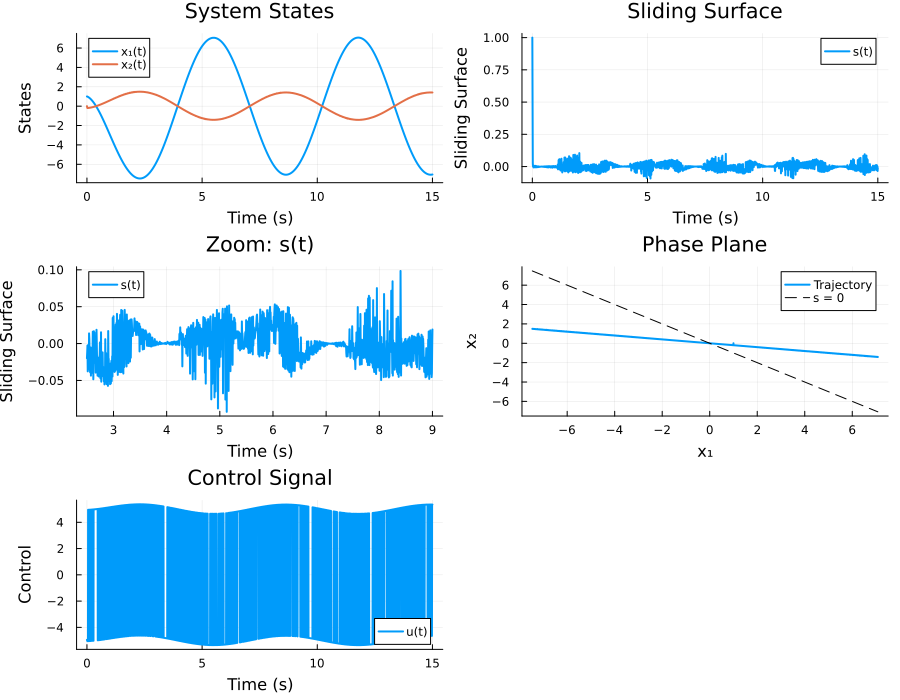
\includegraphics[width=1\textwidth]{img/problem1_6.png}
        \caption{Simulation results for the sliding mode control system.}
        \label{fig:problem1_6}
    \end{figure}
    The simulation shows that the system converges to the sliding mode, but the disturbance \( T_L \) prevents the $x_1 = \omega$ state variable from converging asymptotically to zero.
\end{solution}

\newpage
\begin{problem}{1.7}{problem1_7}

Repeat Exercise 1.6 assuming that only the angular speed \( \omega(t) \) is measured. Design a sliding mode observer to estimate the armature current, ensuring that \( \hat{i}(t) \to i(t) \) as \( t \to \infty \). Simulate the closed-loop control system with this observer. Plot the time histories of the sliding variable, the control input \( u(t) \), the angular speed \( \omega(t) \), the actual current \( i(t) \), and the estimated current \( \hat{i}(t) \).

\end{problem}

\begin{solution}{}{solution1_7}

	Let the observer estimate the state \( \hat{x}_1 \) using:
	\[
		\dot{\hat{x}}_1 = v,
	\]
	and define the observation error:
	\[
		z_1 = \hat{x}_1 - x_1.
	\]

	Taking the derivative:
	\[
		\dot{z}_1 = \dot{\hat{x}}_1 - \dot{x}_1 = v - \left(\frac{k_m}{J}x_2 - \frac{T_L}{J}\right).
	\]

	Define the correction term as:
	\[
		v = -\rho \, \text{sign}(z_1),
	\]
	with a gain satisfying:
	\[
		\rho > \frac{k_m}{J} |x_2| + \frac{|T_L|_{\max}}{J} + \beta, \quad \beta > 0.
	\]

	Thus, the observation error dynamics becomes:
	\[
		\dot{z}_1 = -\frac{k_m}{J} x_2 + \frac{T_L}{J} - \rho \, \text{sign}(z_1),
	\]
	and the Lyapunov analysis gives:
	\[
		z_1 \dot{z}_1 = z_1 \left(-\frac{k_m}{J} x_2 + \frac{T_L}{J} - \rho \, \text{sign}(z_1)\right).
	\]

	On the sliding surface \( z_1 = 0 \), the equivalent control satisfies:
	\[
		\dot{z}_1 = 0 \quad \Rightarrow \quad -\frac{k_m}{J} x_2 + \frac{T_L}{J} + v_{\text{eq}} = 0.
	\]

	Solving for \( x_2 \), we get:
	\[
		x_2 = \frac{T_L}{k_m} + \frac{J}{k_m} v_{\text{eq}}.
	\]

	Since \( T_L \) is unknown, we estimate \( x_2 \) using only \( v_{\text{eq}} \). To approximate \( v_{\text{eq}} \), we use a \emph{low-pass filter}:
	\[
		\tau \dot{\hat{v}}_{\text{eq}} = -\hat{v}_{\text{eq}} - \rho \, \text{sign}(z_1),
	\]
	where \( \tau \) is the filter time constant.\\

    And this is a great achievement, as we have now an estimate of $\dot{x}_1$, in which previously we had an unmatched disturbance. So we can redefine the sliding variable as:
    \[
        s = \dot{\hat{x}}_1 + \lambda x_1
    \]
    for the control purposes.\\

	Additionally, after the reaching time \( t_r \), we estimate:
	\[
		\hat{x}_2(t) \approx \frac{T_L}{k_m} + \frac{J}{k_m}\hat{v}_{\text{eq}}(t).
	\]

    Finally, simulating the same conditions and parameters as in Exercise 1.6, with the new sliding variable and with tho observer gain $\rho_o = 20$, and the filter time constant $\tau = 0.01$, we get the following results:

    \begin{figure}[H]
        \centering
        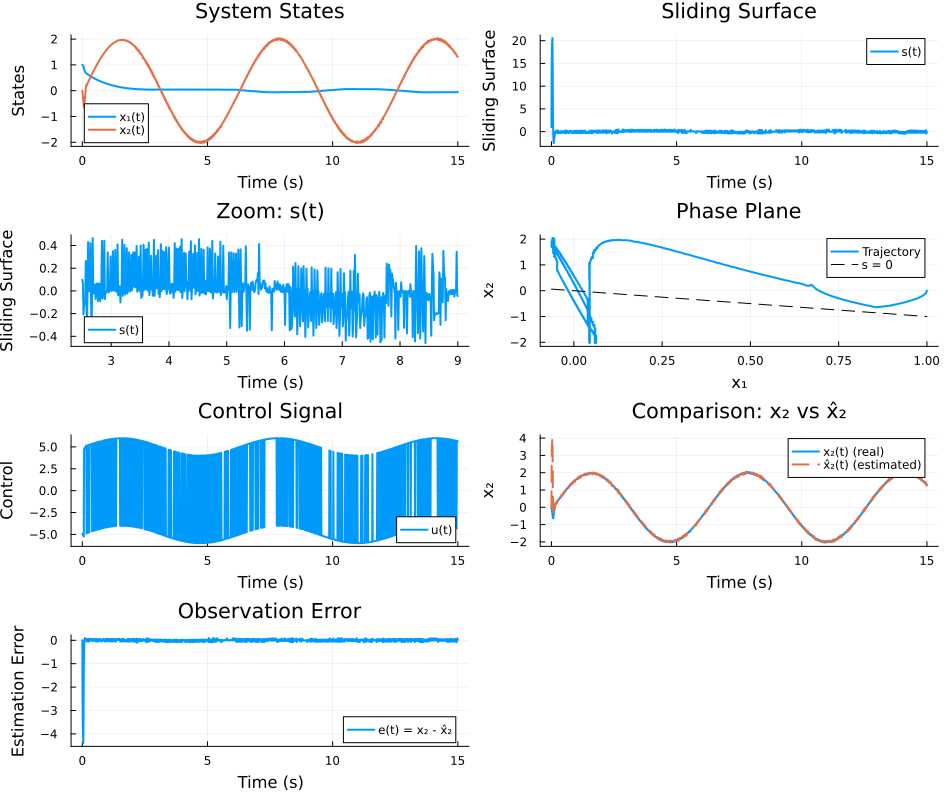
\includegraphics[width=1\textwidth]{img/problem1_7.png}
        \caption{Simulation results for the sliding mode control system with observer.}
        \label{fig:problem1_7}
    \end{figure}

    In the simulation, we observe that the sliding mode observer successfully estimates the armature current \( i(t) \), and the new sliding variable \( s(t) \) converges to zero. A key advantage of this observer is its ability to estimate the state variable \( \dot{x}_1 \), which is crucial for defining the \textit{new} sliding surface. This represents a significant improvement over the previous exercise, where we had to contend with an unmatched disturbance. Now, by effectively \textit{observing} that disturbance through the observer, we are able to compensate for it. The simulation results confirm the convergence of the angular speed \( x_1 = \omega \) to zero, fulfilling the original control objective.

\end{solution}
\newpage
\begin{problem}{2.1}{problem2_1}

Consider the linear system
\[
	\begin{aligned}
		\dot{x} & = Ax + Bu \\
		\sigma  & = Gx
	\end{aligned}
\]
with $\sigma$ as the sliding variable. Find the equivalente control $u_{\text{eq}}$ and the sliding mode equations when
\begin{enumerate}
	\item
	      \[
		      A = \begin{bmatrix}
			      2 & 19 \\
			      3 & 29
		      \end{bmatrix}, \quad B = \begin{bmatrix}
			      2 \\
			      3
		      \end{bmatrix}, \quad \text{and} \quad G = \begin{bmatrix}
			      9 & 12
		      \end{bmatrix}
	      \]
	\item
	      \[
		      A = \begin{bmatrix}
			      1 & 1 & 1 \\
			      0 & 1 & 3 \\
			      1 & 0 & 1
		      \end{bmatrix}, \quad B = \begin{bmatrix}
			      3  & 9  \\
			      1  & -2 \\
			      -1 & 0
		      \end{bmatrix}, \quad \text{and} \quad G = \begin{bmatrix}
			      1 & 29 & 0 \\
			      1 & 12 & 0
		      \end{bmatrix}
	      \]
\end{enumerate}

\end{problem}

\begin{solution}{}{solution2_1}
	\textbf{Finding the equivalent control \( u_{\text{eq}} \):}

	The equivalent control \( u_{\text{eq}} \) is obtained by imposing that the sliding surface remains invariant, i.e., \( \dot{\sigma} = 0 \) on the sliding manifold.

	\begin{enumerate}
		\item First, differentiate \( \sigma \):
		      \[
			      \dot{\sigma} = G\dot{x}
		      \]
		      where \( G \) defines the sliding surface. Substituting the system dynamics \( \dot{x} = Ax + Bu \) yields:
		      \[
			      \dot{\sigma} = G(Ax + Bu) = GAx + GBu
		      \]

		\item On the sliding surface, we require \( \dot{\sigma} = 0 \), which gives:
		      \[
			      0 = GAx + GBu
		      \]

		\item Solving for \( u_{\text{eq}} \) leads to:
		      \[
			      GBu_{\text{eq}} = -GAx \quad \Rightarrow \quad u_{\text{eq}} = -(GB)^{-1}GAx
		      \]
		      assuming that \( GB \) is invertible.

		\item Finally, substituting \( u = u_{\text{eq}} \) into \( \dot{x} = Ax + Bu \) provides the \textbf{sliding mode equations}.
	\end{enumerate}

	\bigskip

	\textbf{Problem (a):}

	\begin{enumerate}
		\item Compute \( GA \), \( GB \), and \( (GB)^{-1} \):
		      \[
			      GA = \begin{bmatrix} 9 & 12 \end{bmatrix}
			      \begin{bmatrix}
				      3 & 19 \\
				      3 & 29
			      \end{bmatrix}
			      = \begin{bmatrix}
				      54 & 519
			      \end{bmatrix}
		      \]

		      \[
			      GB = \begin{bmatrix} 9 & 12 \end{bmatrix}
			      \begin{bmatrix}
				      2 \\ 3
			      \end{bmatrix}
			      = 54
			      \quad \Rightarrow \quad (GB)^{-1} = \frac{1}{54}
		      \]

		\item Find \( u_{\text{eq}} \):
		      \[
			      \begin{aligned}
				      u_{\text{eq}} & = -\frac{1}{54} \begin{bmatrix} 54 & 519 \end{bmatrix}
				      \begin{bmatrix}
					      x_1 \\ x_2
				      \end{bmatrix}                                                         \\
				                    & = -x_1 - \frac{519}{54} x_2
			      \end{aligned}
		      \]

		\item Substitute \( u_{\text{eq}} \) into the system dynamics:
		      \[
			      \begin{aligned}
				      \dot{x} & = Ax + Bu_{\text{eq}}                      \\
				              & = \begin{bmatrix}
					                  3 & 19 \\
					                  3 & 29
				                  \end{bmatrix}
				      \begin{bmatrix}
					      x_1 \\ x_2
				      \end{bmatrix}
				      + \begin{bmatrix}
					        2 \\ 3
				        \end{bmatrix}
				      \left( -x_1 - \frac{519}{54}x_2 \right)              \\
				              & = \begin{bmatrix}
					                  2x_1 + 19x_2 - 2x_1 - 2\frac{519}{54}x_2 \\
					                  3x_1 + 29x_2 - 3x_1 - 3\frac{519}{54}x_2
				                  \end{bmatrix}
			      \end{aligned}
		      \]

		      Therefore, the sliding mode dynamics are:
		      \[
			      \dot{x} = \begin{bmatrix}
				      -0.222x_2 \\
				      0.166x_2
			      \end{bmatrix}
		      \]
	\end{enumerate}

	\bigskip

	\textbf{Problem (b):}

	\begin{enumerate}
		\item Compute \( GA \), \( GB \), and \( (GB)^{-1} \):
		      \[
			      GA = \begin{bmatrix}
				      1 & 29 & 0 \\
				      1 & 12 & 0
			      \end{bmatrix}
			      \begin{bmatrix}
				      1 & 1 & 1 \\
				      0 & 1 & 3 \\
				      1 & 0 & 1
			      \end{bmatrix}
			      = \begin{bmatrix}
				      1 & 30 & 88 \\
				      1 & 13 & 37
			      \end{bmatrix}
		      \]

		      \[
			      GB = \begin{bmatrix}
				      1 & 29 & 0 \\
				      1 & 12 & 0
			      \end{bmatrix}
			      \begin{bmatrix}
				      3  & 9  \\
				      1  & -2 \\
				      -1 & 0
			      \end{bmatrix}
			      = \begin{bmatrix}
				      32 & -49 \\
				      15 & -15
			      \end{bmatrix}
		      \]

		      \[
			      (GB)^{-1} = \frac{1}{255}
			      \begin{bmatrix}
				      -15 & 49 \\
				      -15 & 32
			      \end{bmatrix}
		      \]

		\item Find \( u_{\text{eq}} \):
		      \[
			      \begin{aligned}
				      u_{\text{eq}} & = - (GB)^{-1} GAx \\
				                    & = -\frac{1}{255}
				      \begin{bmatrix}
					      -15 & 49 \\
					      -15 & 32
				      \end{bmatrix}
				      \begin{bmatrix}
					      1 & 30 & 88 \\
					      1 & 13 & 37
				      \end{bmatrix}
				      \begin{bmatrix}
					      x_1 \\x_2\\x_3
				      \end{bmatrix}                    \\
				                    & = \frac{1}{15}
				      \begin{bmatrix}
					      -2 & -11 & -29 \\
					      -1 & 2   & 8
				      \end{bmatrix}
				      \begin{bmatrix}
					      x_1 \\x_2\\x_3
				      \end{bmatrix}
			      \end{aligned}
		      \]

		\item Substitute \( u_{\text{eq}} \) into the system dynamics:
		      \[
			      \begin{aligned}
				      \dot{x} & = Ax + Bu_{\text{eq}} \\
				              & = \begin{bmatrix}
					                  1 & 1 & 1 \\
					                  0 & 1 & 3 \\
					                  1 & 0 & 1
				                  \end{bmatrix}
				      \begin{bmatrix}
					      x_1 \\x_2\\x_3
				      \end{bmatrix}
				      + \frac{1}{15}
				      \begin{bmatrix}
					      3  & 9  \\
					      1  & -2 \\
					      -1 & 0
				      \end{bmatrix}
				      \begin{bmatrix}
					      -2 & -11 & -29 \\
					      -1 & 2   & 8
				      \end{bmatrix}
				      \begin{bmatrix}
					      x_1 \\x_2\\x_3
				      \end{bmatrix}                  \\
				              & = \frac{1}{15}
				      \begin{bmatrix}
					      0  & 0  & 0  \\
					      0  & 0  & 0  \\
					      17 & 11 & 44
				      \end{bmatrix}
				      \begin{bmatrix}
					      x_1 \\x_2\\x_3
				      \end{bmatrix}
			      \end{aligned}
		      \]
                Therefore, the sliding mode dynamics are:
                \[
                    \dot{x} = \begin{bmatrix}
                        0 \\
                        0 \\
                        \frac{17}{15}x_1 + \frac{11}{15}x_2 + \frac{44}{15}x_3
                    \end{bmatrix}
                \]
	\end{enumerate}

\end{solution}

\newpage
\begin{problem}{2.1}{problem2_1}

Consider the system given by
\[
	\begin{aligned}
		\dot{x}_1 & = x_1 + x_2 + u_1 + 10u_2                  \\
		\dot{x}_2 & = x_2 + 3x_3 + u_1 - 2u_2                  \\
		\dot{x}_3 & = x_1 + x_3 - u_1                          \\
		\sigma_1  & = x_1 + 10x_2, \quad \sigma_2 = x_1 + 5x_2
	\end{aligned}
\]
Find the system dynamics in the sliding mode $\sigma_1 = \sigma_2 = 0$.
\end{problem}

\begin{solution}{}{solution2_1}
	\begin{enumerate}
		\item First, we put the system in state-space form, so it can be solved as the previous problem:
		      \[
			      \begin{aligned}
				      \dot{x} & = Ax + Bu, \quad \sigma = Gx \\
				      A       & = \begin{bmatrix}
					                  1 & 1 & 0 \\
					                  0 & 1 & 3 \\
					                  1 & 0 & 1
				                  \end{bmatrix}, \quad
				      B       = \begin{bmatrix}
					                1  & 10 \\
					                1  & -2 \\
					                -1 & 0
				                \end{bmatrix}, \quad
				      G       = \begin{bmatrix}
					                1 & 10 \\
					                1 & 5
				                \end{bmatrix}
			      \end{aligned}
		      \]
		\item Compute \( GA \), \( GB \), and \( (GB)^{-1} \):
		      \[
			      GA = \begin{bmatrix}
				      1 & 11 & 31 \\
				      1 & 6  & 16
			      \end{bmatrix}
		      \]
		      \[
			      GB = \begin{bmatrix}
				      11 & -10 \\
				      6  & 0
			      \end{bmatrix}
		      \]
		      \[
			      (GB)^{-1} = \frac{1}{60}
			      \begin{bmatrix}
				      0  & 10 \\
				      -6 & 11
			      \end{bmatrix}
		      \]


		\item Find \( u_{\text{eq}} \):
		      \[
			      \begin{aligned}
				      u_{\text{eq}} & = - (GB)^{-1} GAx \\
				                    & = -\frac{1}{60}
				      \begin{bmatrix}
					      0  & 10 \\
					      -6 & 11
				      \end{bmatrix}
				      \begin{bmatrix}
					      1 & 11 & 31 \\
					      1 & 6  & 16
				      \end{bmatrix}
				      \begin{bmatrix}
					      x_1 \\ x_2 \\ x_3
				      \end{bmatrix}                  \\
				                    & = -\frac{1}{60}
				      \begin{bmatrix}
					      10 & 60 & 160 \\
					      5  & 0  & -10
				      \end{bmatrix} \begin{bmatrix}
					                    x_1 \\ x_2 \\ x_3
				                    \end{bmatrix}
			      \end{aligned}
		      \]

		\item Substitute \( u_{\text{eq}} \) into the system dynamics:
		      \[
			      \begin{aligned}
				      \dot{x} & = Ax + Bu_{\text{eq}}                             \\
				              & = \begin{bmatrix}
					                  1 & 1 & 0 \\
					                  0 & 1 & 3 \\
					                  1 & 0 & 1
				                  \end{bmatrix} \begin{bmatrix}
					                                x_1 \\ x_2 \\ x_3
				                                \end{bmatrix}
				      - \frac{1}{60} \begin{bmatrix}
					                     1  & 10 \\
					                     1  & -2 \\
					                     -1 & 0
				                     \end{bmatrix} \begin{bmatrix}
					                                   10 & 60 & 160 \\
					                                   5  & 0  & -10
				                                   \end{bmatrix} \begin{bmatrix}
					                                                 x_1 \\ x_2 \\ x_3
				                                                 \end{bmatrix} \\
				              & = \frac{1}{6}\begin{bmatrix}
					                             0 & 0 & 0  \\
					                             0 & 0 & 0  \\
					                             7 & 1 & 22
				                             \end{bmatrix} \begin{bmatrix}
					                                           x_1 \\ x_2 \\ x_3
				                                           \end{bmatrix}
			      \end{aligned}
		      \]

		      Therefore, the sliding mode dynamics are:
		      \[
			      \dot{x} = \begin{bmatrix}
				      0 \\
				      0 \\
				      \frac{7}{6}x_1 + \frac{1}{6}x_2 + \frac{22}{6}x_3
			      \end{bmatrix}
		      \]
	\end{enumerate}
\end{solution}

\newpage

\begin{problem}{2.3}{problem2_3}
Consider the DC-DC buck converter in Fig. 2.19 which belongs to the class of attenuation circuits; the corresponding dynamic equations are given by:
$$
	\begin{aligned}
		L \frac{d i}{d t} & =-v+u V_{i n}  \\
		C \frac{d v}{d t} & =i-\frac{v}{R}
	\end{aligned}
$$
where $i$ is the current through the inductor $L, v$ is the voltage across the capacitor $C$, $V_{i n}$ is the input voltage, and $u \in\{0,1\}$ is the switching control signal. The goal is to stabilize the output voltage $v$ at the desired level $v_d$. This goal is to be achieved via stabilization of the inductor current $i$ at the desired level $i_d=\frac{v_d}{R}$ using sliding mode control, for this purpose:
(a) Setting $\sigma=i-i_d$ and using the control input $u=\frac{1}{2}(1-\operatorname{sign}(\sigma))$, find the equivalent control and the sliding mode dynamics.
(b) Considering $L=20 \mathrm{mH}, C=20 \mu \mathrm{~F}, R=30 \Omega$, $V_{i n}=15 \mathrm{~V}, v_d=10 \mathrm{~V}$, and the initial conditions $i(0)=0.1 \mathrm{~A}$ and $v(0)=5 \mathrm{~V}$, confirm the efficacy of the controller by simulations.
\end{problem}
\newpage
\begin{problem}{2.5}{problem2_5}
Using the sliding variable $\sigma = x_1$ and the control $u = -\text{sign}(\sigma)$, find the sliding mode equation for the systems given below, by using the equivalent control method and Filippov method for the cases:

\begin{itemize}
	\item[(a)]
		\begin{align*}
			\dot{x}_1 & = u             \\
			\dot{x}_2 & = (2u^2 - 1)x_2
		\end{align*}
	\item[(b)]
		\begin{align*}
			\dot{x}_1 & = u             \\
			\dot{x}_2 & = (u - 2u^3)x_2
		\end{align*}
	\item[(c)]
		\begin{align*}
			\dot{x}_1 & = u             \\
			\dot{x}_2 & = (u - 2u^2)x_2
		\end{align*}
\end{itemize}
\end{problem}

\begin{solution}{}{solution2_5}
	\textbf{(a)}
	\begin{enumerate}
		\item \textbf{Equivalent control Method:}

		      The sliding surface is defined as $\sigma = x_1$. In sliding mode, we require:
		      \begin{align*}
			      \sigma       & = 0, \\
			      \dot{\sigma} & = 0.
		      \end{align*}
		      Since $\dot{\sigma} = \dot{x}_1 = u$, imposing $\dot{\sigma} = 0$ gives:
		      \[
			      u_{eq} = 0.
		      \]

		      Substituting $u_{eq} = 0$ into the second equation:
		      \begin{align*}
			      \dot{x}_2 & = (2(0)^2 - 1)x_2 \\
			                & = -x_2.
		      \end{align*}

		      Thus, the sliding mode dynamics under the equivalent control method are:
		      \[
			      \dot{x}_2 = -x_2.
		      \]
		\item \textbf{Filippov Method:}

		      The actual control law is $u = -\text{sign}(x_1)$, leading to discontinuities at $x_1 = 0$. To apply Filippov's method, we examine the system's behavior on both sides:

		      \begin{itemize}
			      \item If $x_1 > 0$, then $u = -1$.
			      \item If $x_1 < 0$, then $u = +1$.
		      \end{itemize}

		      Substituting into the dynamics:
		      \begin{itemize}
			      \item For $u = -1$:
			            \begin{align*}
				            \dot{x}_1 & = -1,                  \\
				            \dot{x}_2 & = (2(1) - 1)x_2 = x_2.
			            \end{align*}

			      \item For $u = +1$:
			            \begin{align*}
				            \dot{x}_1 & = 1,                   \\
				            \dot{x}_2 & = (2(1) - 1)x_2 = x_2.
			            \end{align*}
		      \end{itemize}

		      The Filippov convex combination requires choosing a mixture such that $\dot{x}_1 = 0$:
		      \[
			      (1-\alpha)(-1) + \alpha(1) = 0 \quad \Rightarrow \quad \alpha = \frac{1}{2}.
		      \]

		      Thus, the sliding dynamics for $x_2$ are:
		      \[
			      \dot{x}_2 = x_2.
		      \]

		\item \textbf{Final Results:}
		      \begin{itemize}
			      \item Equivalent Control Method: $\dot{x}_2 = -x_2$
			      \item Filippov Method: $\dot{x}_2 = x_2$
		      \end{itemize}
	\end{enumerate}
	\textbf{(b)}
	\begin{enumerate}
		\item \textbf{Equivalent control Method:}
		      \[
			      \dot{\sigma} = \dot{x}_1 = u = 0 \Rightarrow u_{eq} = 0.
		      \]
		      Substituting $u_{eq} = 0$:
		      \begin{align*}
			      \dot{x}_1 & = 0, \\
			      \dot{x}_2 & = 0.
		      \end{align*}
		\item \textbf{Filippov Method:}
		      \begin{itemize}
			      \item For $u = -1$:
			            \begin{align*}
				            \dot{x}_1 & = -1, \\
				            \dot{x}_2 & = x_2
			            \end{align*}
			      \item For $u = +1$:
			            \begin{align*}
				            \dot{x}_1 & = 1,   \\
				            \dot{x}_2 & = -x_2
			            \end{align*}
		      \end{itemize}
		      Then, is trivial to see that $\alpha = \frac{1}{2}$ again, so we have:
		      \[
			      \dot{x}_2 = (1-\alpha)(x_2) - \alpha x_2 = 0
		      \]
		\item \textbf{Final Results:}
		      \begin{itemize}
			      \item Equivalent Control Method: $\dot{x}_2 = 0$
			      \item Filippov Method: $\dot{x}_2 = 0$
		      \end{itemize}
	\end{enumerate}
	\textbf{(c)}
	\begin{enumerate}
		\item \textbf{Equivalent control Method:}
		      \[
			      \dot{\sigma} = \dot{x}_1 = u = 0 \Rightarrow u_{eq} = 0.
		      \]
		      Substituting $u_{eq} = 0$:
		      \begin{align*}
			      \dot{x}_1 & = 0, \\
			      \dot{x}_2 & = 0.
		      \end{align*}
		\item \textbf{Filippov Method:}
		      \begin{itemize}
			      \item For $u = -1$:
			            \begin{align*}
				            \dot{x}_1 & = -1,    \\
				            \dot{x}_2 & = -3 x_2
			            \end{align*}
			      \item For $u = +1$:
			            \begin{align*}
				            \dot{x}_1 & = 1,   \\
				            \dot{x}_2 & = -x_2
			            \end{align*}
		      \end{itemize}
		      Then, is trivial to see that $\alpha = \frac{1}{2}$ again, so we have:
		      \[
			      \dot{x}_2 = (1-\alpha)(-3x_2) - \alpha x_2 = -2x_2
		      \]
		\item \textbf{Final Results:}
		      \begin{itemize}
			      \item Equivalent Control Method: $\dot{x}_2 = 0$
			      \item Filippov Method: $\dot{x}_2 = -2x_2$
		      \end{itemize}
	\end{enumerate}


\end{solution}

% \bibliographystyle{apalike}
% \bibliography{references}

\end{document}